% !TEX root = ../../seminar.tex

\subsubsection{Research Question}

The question a study is designed to answer is called research question \cite{Vickers}. It should be an answerable question that addresses a relevant issue in the research area \cite{Dyba2005}. To produce questions which drive knowledge further, a deep understanding of the topics that have already been studied is needed.
The questions that arise during the acquisition of knowledge, which cannot be answered by means of EBSE, are likely appropriate questions for further research \cite{Farrugia2009}.

There are two general classes of research questions: qualitative and quantitative questions. Qualitative research states questions which report, describe, or explore a subject \cite[p. 139-141]{Creswell2014}. The issues computer science students are confronted with are rather of quantitative nature than qualitative (e.g. \q{Is database engine X faster than database engine Y?}). These problems are different from the problems researchers commonly investigate (see issue \ref{itm:issue7} in table \ref{table:issuesEBSE}) \cite{Rainer2006}. Therefore, this work focuses on quantitative research questions. \q{Quantitative research questions inquire about the relationships among variables} \cite[p. 143]{Creswell2014} and quantitative hypotheses emerge from them.

Shaw provides a model where she categorizes research questions from software engineering papers in five types to understand the structure of research questions \cite{Shaw2002}. 

To design a good research question, Haynes coined the acronym PICO: Population, Intervention, Comparison group, and Outcome \cite{BrianHaynes2006}. Sometimes Time is added as fifth component, when it is important over which time frame the study is conducted. See the left box in figure \ref{fig:PICOT_FINER}. A research question structured with the PICOT approach supports in restricting the research question and thereby directs hypotheses and study. By restricting the research question researchers can limit bias and increase the internal validity of the study. A too narrow question may lead to decreased external validity \cite{Farrugia2009}. 

Before PICOT Sackett and colleagues suggested that good research questions consist of three components: Intervention, Context and Outcome \cite{Sackett2000}. This is a more coarse grained decomposition than PICOT. Dyb{\aa} \etal displayed a fitting example for this template in software engineering: \q{Does pair programming lead to improved code quality when practiced by professional software developers?} \cite[p. 60]{Dyba2005} In this example, the intervention (technology) is pair programming, the context of interest are professional software developers, and the outcome (effect) is improved code quality \cite{Dyba2005}. To verify the quality of a research question Hulley \etal suggest the use of the FINER criteria. It highlights key aspects of the question and thereby provides new perspective to the proposed study. The FINER criteria consists of: Feasible, Interesting, Novel, Ethical, and Relevant \cite{Farrugia2009}. A more detailed view of the FINER criteria can be seen in the right box of figure \ref{fig:PICOT_FINER}.
\begin{figure}
	\centering
	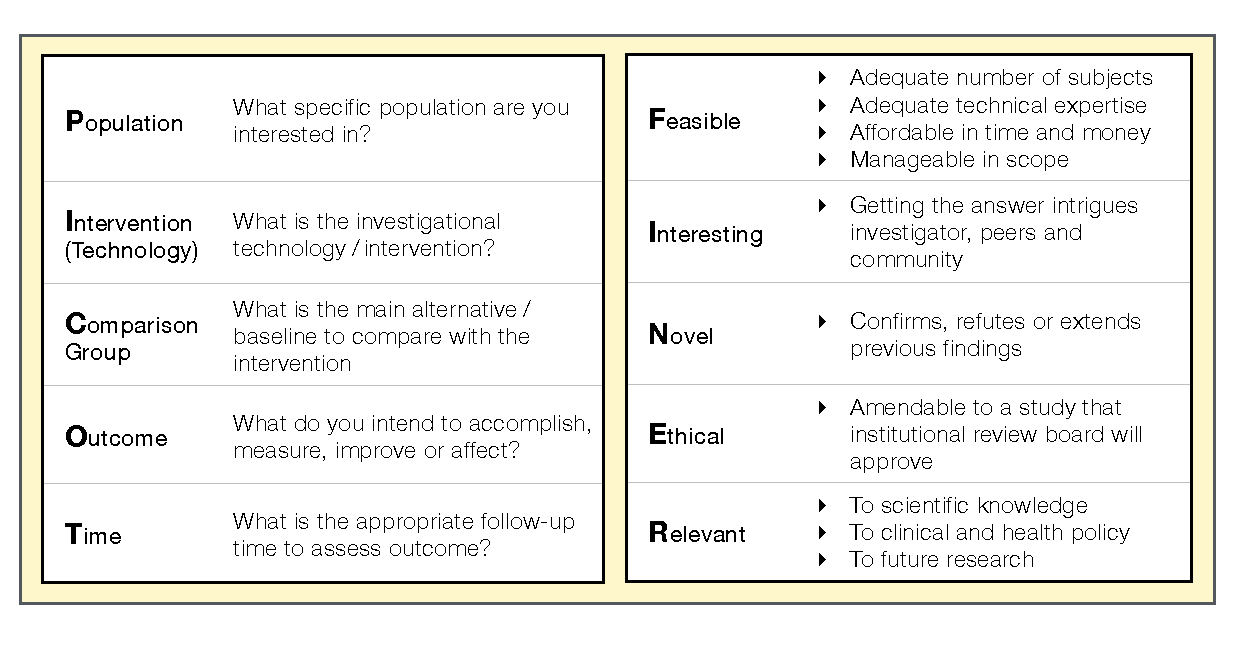
\includegraphics[width=12cm]{figures/picot_finer.pdf}
	\caption{PICOT criteria adjusted to computer science research \cite{Farrugia2009} and FINER criteria for a good research question \cite{Farrugia2009}.}
	\label{fig:PICOT_FINER}
\end{figure}

